\documentclass[a4paper,10pt,twocolumn]{ltjsarticle}
\usepackage[haranoaji]{luatexja-preset}
\usepackage[top=18mm,bottom=20mm,left=17mm,right=17mm,columnsep=8mm]{geometry}
\usepackage{graphicx,booktabs,array,caption,enumitem,xcolor,tikz}
\usetikzlibrary{shapes.geometric}
\setlength{\parindent}{1\zw}
\renewcommand{\baselinestretch}{1.0}
\setlength{\parskip}{0pt}
\renewcommand{\thesection}{\arabic{section}.}
\renewcommand{\thesubsection}{\arabic{section}.\arabic{subsection}.}
\makeatletter
\renewcommand{\section}{\@startsection{section}{1}{\z@}{1.1\Cvs \@plus.4\Cdp \@minus.2\Cdp}{.5\Cvs \@plus.2\Cdp}{\normalfont\gtfamily\bfseries\large}}
\renewcommand{\subsection}{\@startsection{subsection}{2}{\z@}{.8\Cvs \@plus.3\Cdp \@minus.2\Cdp}{.3\Cvs \@plus.1\Cdp}{\normalfont\gtfamily\bfseries\normalsize}}
\makeatother
\captionsetup{font={small,sf},labelsep=space,justification=raggedright,singlelinecheck=false,skip=3pt}
\captionsetup[table]{position=top}
\setlist[itemize]{leftmargin=1.2\zw,itemsep=0pt,topsep=2pt,parsep=0pt}
\setlength{\textfloatsep}{8pt plus 2pt minus 2pt}
\setlength{\floatsep}{8pt plus 2pt minus 2pt}
\setlength{\intextsep}{8pt plus 2pt minus 2pt}
\pagestyle{plain}
\raggedbottom
\begin{document}
\twocolumn[{
\noindent\fbox{\gtfamily\small\ 生成AI論文\ }\par\medskip
\begin{center}
{\gtfamily\bfseries\LARGE 日本の子どもは算数・数学が好きなのか：TIMSS 2023で小4・中2を国際比較する$^{\dagger}$}\par\medskip
{\gtfamily\bfseries\large 「とても好き」「とても自信がある」児童生徒の割合と国・地域間の関連}\par\medskip
{\normalsize EduData調査研究グループ$^{*1}$・教育データサイエンス解析班$^{*2}$}\par
{\small オープン教育統計推進プロジェクト$^{*1}$・初等中等STEM教育データ基盤ユニット$^{*2}$}
\end{center}\smallskip
\noindent\begin{minipage}{\textwidth}\small 本研究は，TIMSS 2023の公表値から，算数・数学を「とても好き」「とても自信がある」と答えた児童生徒の割合を，小4（58の国・地域）と中2（43の国・地域）で整理した．日本は平均得点が高い一方，小4の「とても好き」は22\%（単純平均44.34\%）で台湾，韓国と並ぶ55〜57番目，「とても自信あり」は14\%で最も低かった．中2も「とても好き」10\%，「とても自信あり」4\%と低い位置にあった．小4では「とても好き」の割合が高い国・地域ほど「とても自信あり」の割合も高かった（\textit{r}=.45，\textit{BF}\textsubscript{10}=61.78）．これらは自己申告にもとづく集計値の関連であり，個々の児童生徒の因果を示さない．\par\smallskip
\noindent{\gtfamily キーワード：}TIMSS 2023，算数・数学，学習意欲，自信，国際比較\end{minipage}\medskip
}]
\let\thefootnote\relax
\footnotetext{\footnotesize 2026年10月執筆\\ $^{\dagger}$Do Children in Japan Like Mathematics? A Cross-National Comparison of Grade 4 and Grade 8 Students in TIMSS 2023\\ $^{*1}$ Open Education Data Project, Tokyo, Japan\quad $^{*2}$ Educational Data Science Unit, Tokyo, Japan}
\section{はじめに}
\subsection{研究の背景}
算数・数学への態度は，動機づけの研究で扱われてきた．Wigfield and Eccles (2000)は期待と価値から達成の動機づけを説明する理論を示し，Bandura (1997)は自己効力感の理論を示した．Pekrun (2006)は学業での感情を統制と価値の評価から説明する．ただし，これらは個人についての理論である．国際比較では，Shen and Tam (2008)がTIMSSの3回の調査から，得点と自己認識の国をまたぐ関係が逆説的であることを論じ，Lee and Stankov (2018)はTIMSSとPISAから非認知的な要因と学力の関連を検討した．また，Chen et al. (1995)は，東アジアと北米の生徒で評定尺度への回答の仕方が異なることを示している．

TIMSSはIEAが行う算数・数学と理科の国際調査で，Mullis et al. (2020)が2019年の結果を，IEA (2024)が2023年の結果を報告している．本研究では，2023年の公表値から，日本の小4・中2の態度の位置を整理する．
\subsection{リサーチクエスチョン}
本研究の目的は，TIMSS 2023の公表値から，算数・数学への態度の国・地域による違いと日本の位置を記述することである．
\begin{itemize}
\item RQ1：「とても好き」「とても自信がある」と答えた児童生徒の割合は，国・地域によってどう違い，日本はどこに位置するか．
\item RQ2：小4で「とても好き」な児童の割合が高い国・地域ほど，「とても自信がある」児童の割合も高いか．
\end{itemize}
\section{調査対象および分析方法}
IEA (2024)が公表した表のExcelから，「好き」「自信」「価値」（価値は中2のみ）の尺度で「とても」肯定する児童生徒と肯定しない児童生徒の割合（\%），2群の平均得点の差，国・地域の平均得点を機械的に取り込んだ．対象は小4が58，中2が43の国・地域で，国際平均とベンチマーク参加は除いた．小4と中2は別の変数とし，学年をまたいで混ぜていない．平均は国・地域の単純平均である．

ピアソンの\textit{r}と95\%信頼区間，スピアマンの\textit{ρ}，\textit{p}，JZSベイズファクター\textit{BF}\textsubscript{10}を求め，\textit{BF}\textsubscript{10}が3を超えれば関連を支持，1/3未満なら関連がないことを支持とみなした．17指標の全136組を探索したため，ボンフェローニの基準（.05÷136）を併せて見た．同じ尺度の2つの割合のように計算でつながる組は結果としない．
\begin{table*}[!t]
\caption{主要指標の基本記述統計量}
\centering\small
\begin{tabular}{>{\raggedright\arraybackslash}p{9.2cm}rrrrrr}
\toprule
指標 & \textit{K} & 平均 & \textit{SD} & 中央値 & 最小 & 最大 \\
\midrule
小4・とても好き(\%) & 58 & 44.3 & 16.4 & 40.0 & 21.0 & 80.0 \\
小4・好きでない(\%) & 58 & 23.9 & 11.7 & 25.0 & 5.0 & 48.0 \\
小4・好き層と好きでない層の得点差 & 58 & 31.8 & 11.9 & 29.5 & 9.0 & 57.0 \\
小4・とても自信あり(\%) & 58 & 27.2 & 6.2 & 28.0 & 14.0 & 41.0 \\
小4・自信なし(\%) & 58 & 31.3 & 5.9 & 31.0 & 19.0 & 45.0 \\
小4・自信あり層と自信なし層の得点差 & 58 & 87.8 & 15.4 & 87.0 & 50.0 & 126.0 \\
小4・平均得点 & 58 & 503.2 & 56.0 & 514.5 & 362.0 & 615.0 \\
中2・とても好き(\%) & 43 & 21.3 & 12.3 & 18.0 & 7.0 & 56.0 \\
中2・好きでない(\%) & 43 & 46.3 & 15.1 & 49.0 & 11.0 & 69.0 \\
中2・好き層と好きでない層の得点差 & 43 & 49.5 & 22.2 & 50.0 & -2.0 & 89.0 \\
中2・とても自信あり(\%) & 43 & 12.9 & 3.5 & 13.0 & 4.0 & 20.0 \\
中2・自信なし(\%) & 43 & 55.4 & 6.9 & 54.0 & 43.0 & 74.0 \\
中2・自信あり層と自信なし層の得点差 & 43 & 109.1 & 20.1 & 111.0 & 50.0 & 167.0 \\
中2・とても価値ありと考える(\%) & 43 & 34.4 & 14.7 & 31.0 & 12.0 & 71.0 \\
中2・価値を感じない(\%) & 43 & 24.3 & 9.2 & 25.0 & 7.0 & 45.0 \\
中2・価値あり層と価値なし層の得点差 & 43 & 39.8 & 18.2 & 41.0 & -8.0 & 84.0 \\
中2・平均得点 & 43 & 473.5 & 70.6 & 488.0 & 263.0 & 605.0 \\
\bottomrule
\end{tabular}
\par\smallskip{\footnotesize 注）単位は\%，\textit{K}は観測数（国・地域・区分）．}
\end{table*}
\begin{table*}[!t]
\caption{主要指標間のピアソンの相関係数と，ベイズファクター}
\centering\small
\begin{tabular}{>{\raggedright\arraybackslash}p{6.4cm}>{\raggedright\arraybackslash}p{6.4cm}rrr}
\toprule
指標 \textit{X} & 指標 \textit{Y} & \textit{r} & \textit{p} & \textit{BF}\textsubscript{10} \\
\midrule
小4・とても好き(\%) & 小4・とても自信あり(\%) & .45 & < .001 & 61.78 \\
小4・とても好き(\%) & 小4・好きでない(\%) & −.97 & < .001 & >1000 \\
小4・とても好き(\%) & 小4・好き層と好きでない層の得点差 & .27 & = .040 & 0.84 \\
小4・とても好き(\%) & 小4・自信なし(\%) & −.36 & = .005 & 5.18 \\
小4・とても好き(\%) & 小4・自信あり層と自信なし層の得点差 & −.45 & < .001 & 51.90 \\
\bottomrule
\end{tabular}
\par\smallskip{\footnotesize 注）\textit{BF}\textsubscript{10}はJZSベイズファクター（3を超えれば関連を支持，1/3を下回れば関連がないことを支持）．全ペアの探索の一部を載せた．}
\end{table*}
\section{結果}
RQ1について，小4で「とても好き」と答えた児童の割合は21\%から80\%（単純平均44.34\%，中央値40.0\%）にわたり，高いのはウズベキスタン（80\%），アルバニア（77\%），コソボ（74\%）であった．日本は22\%で，台湾，韓国と同じ値（55〜57番目）であり，「好きでない」は42\%で3番目に高かった．「とても自信あり」は14\%から41\%（平均27.16\%）で，日本の14\%は最も低かった．中2の「とても好き」は7\%から56\%（平均21.26\%，中央値18.0\%）で，日本は10\%（同じ値が5つ，より低い国・地域が4つ），「好きでない」は59\%であった．中2の「とても自信あり」は4\%から20\%（平均12.93\%）で，日本の4\%はマレーシアと並んで最も低く，「自信なし」の74\%は最も高かった．中2の「とても価値あり」も日本は13\%（平均34.37\%）で下から2番目であった．一方，日本の平均得点は小4が591点（5番目），中2が595点（4番目）であった．

RQ2について，小4の「とても好き」と「とても自信あり」の割合の間には中程度の正の相関が見られた（\textit{r}=.45，95\%CI [.22, .64]，\textit{ρ}=.42，\textit{n}=58，\textit{p}<.001，\textit{BF}\textsubscript{10}=61.78）．\textit{p}は約.00033で，136組のボンフェローニ基準（約.00037）をわずかに満たした（補正後の\textit{p}は約.045で，境界に近い）．日本を除いても\textit{r}=.43（\textit{n}=57），1つずつ除いた範囲は.41から.50であった．両方が高い例はウズベキスタン（80\%，40\%），両方が低い例は日本であったが，ブルガリア（50\%，39\%）のように「好き」が中位より上で「自信」も高い国もあった．

補足として，中2では小4のような関連は見られなかった（\textit{r}=.09，95\%CI [−.22, .38]，\textit{n}=43，\textit{BF}\textsubscript{10}=0.14）．\textit{BF}\textsubscript{10}は関連がないことを支持するが，信頼区間は中程度の正の関連を除けない．両学年がそろう37の国・地域に絞ると，\textit{r}は小4で.43，中2で.26であった．また，小4の「とても好き」の割合は国・地域の平均得点と負の相関を示し（\textit{r}=−.65，95\%CI [−.78, −.47]，\textit{ρ}=−.75，\textit{BF}\textsubscript{10}>1000），中2も同じ向きであった（\textit{r}=−.67）．一方，各国・地域の中では，小4の「とても好き」な児童の平均得点は「好きでない」児童より9点から57点（平均31.81点）高かった．
\begin{figure}[t]\centering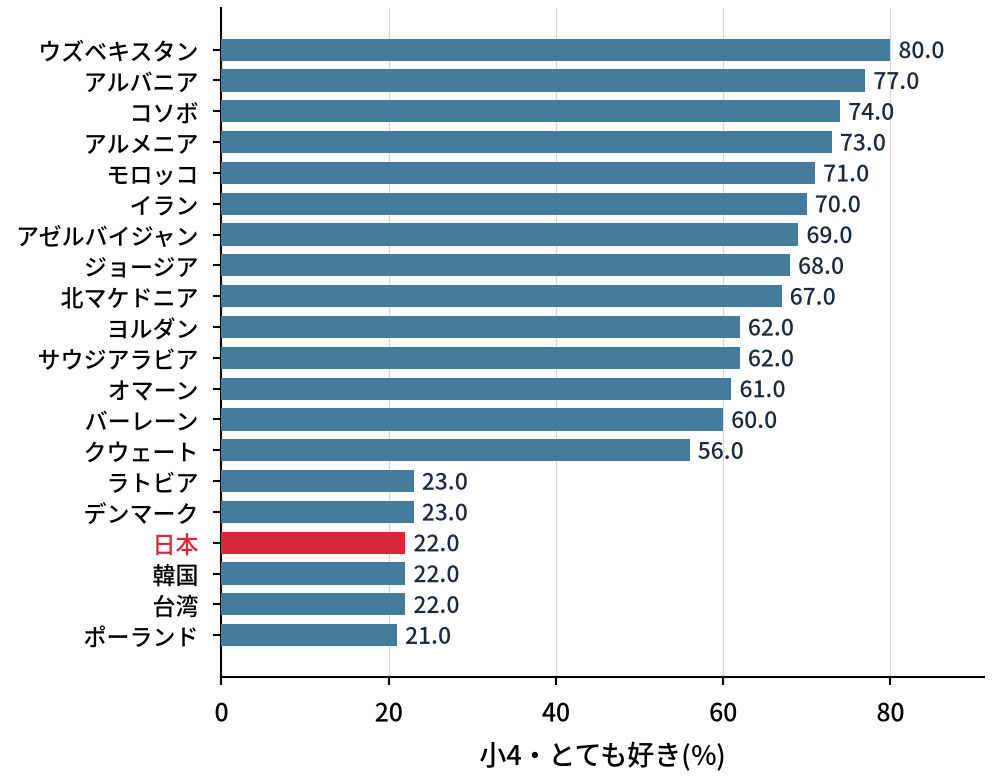
\includegraphics[width=\columnwidth]{chart_timss2023_student_attitudes.png}\caption{小4・とても好き(\%)の値の比較（上位・下位と日本を抜粋）．赤が日本}\end{figure}
\begin{figure}[t]\centering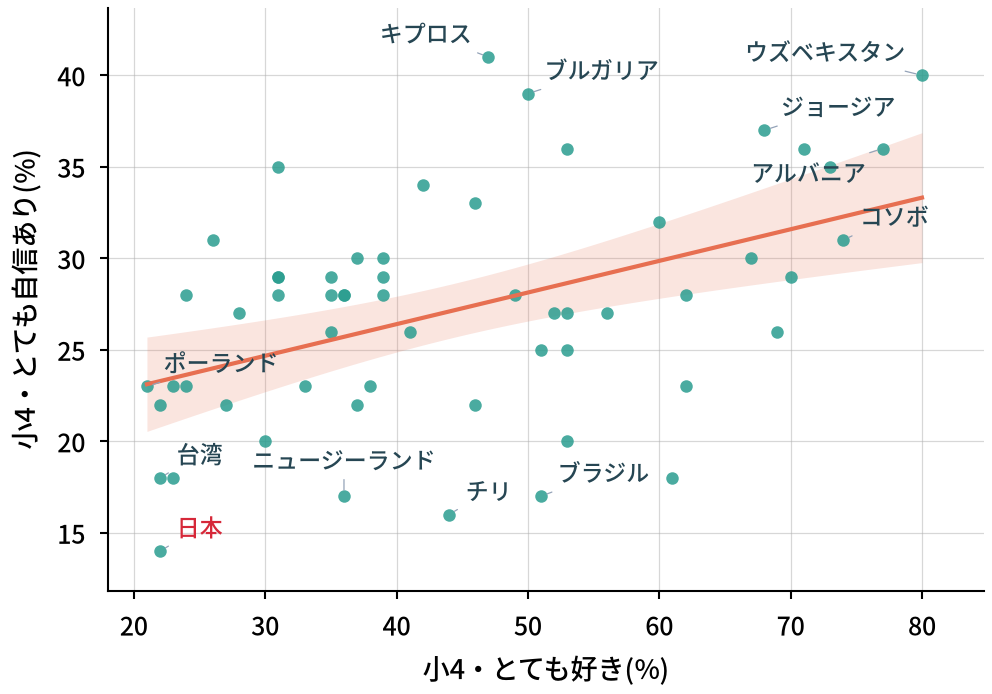
\includegraphics[width=\columnwidth]{chart_secondary_timss2023_student_attitudes.png}\caption{小4・とても好き(\%)と小4・とても自信あり(\%)の関連（回帰直線と，その平均の95\%信頼区間の帯，n=58）}\end{figure}
\section{考察}
RQ1の結果，日本は小4・中2とも平均得点が上位にある一方，「とても好き」「とても自信あり」の割合は下位にあり，自信は両学年で最も低い水準であった．これはIEA (2024)の表の範囲で確かめられることである．Mullis et al. (2020)は2019年の結果を報告しているが，本稿は過去の調査と比べていない．

RQ2では，小4の国・地域の間で「好き」と「自信」の割合に中程度の正の関連が見られた．これはWigfield and Eccles (2000)やPekrun (2006)が個人について論じた期待，価値，感情の結びつきと，向きとしては矛盾しない．しかし，Robinson (1950)が示したように，集計値の関連から，好きな児童ほど自信があるとは言えない（生態学的誤謬）．中2の43の国・地域では小4のような関連は見られなかったが，両学年がそろう37の国・地域では中2の関連（.26）は小4（.43）より弱いものの，.09ほど小さくはなく，国・地域の集合の違いも影響していたと考えられる．なお「とても」は尺度の上位区分の割合であり，中間の回答は見えない．

平均得点と「とても好き」の割合の負の関連は，Shen and Tam (2008)が論じた逆説的な関係と同じ向きであり，国の中では好きな群の得点が高いという結果と食い違う．この食い違いには，Chen et al. (1995)が示した回答の仕方の違いや，Marsh and Hau (2003)が学校内で論じた比較の対象による自己概念の違いのように，国ごとに異なる基準で自分を評価している可能性のほか，教育課程や質問文の翻訳，経済水準の違いも考えられる．Lee and Stankov (2018)も非認知的な要因と学力の関連を国際調査から検討しているが，本研究の説明は仮説にとどまり，このデータでは検証できない．また，群の平均得点の差は，好きになることが得点を高めることを意味しない．Bandura (1997)の自己効力感は個人の経験にもとづく概念であり，日本の自信の低さが実際の効力感の低さか，控えめに答える傾向かは区別できない．

得点が高くても「とても好き」「とても自信がある」と答える児童生徒が少ないという事実を，校内で話し合う材料にすることは考えられるが，その効果は確かめられていない．

本研究の限界は，(1)集計値のみで個人の因果を特定できないこと，(2)自己申告で国により回答の傾向が異なること，(3)標本調査の公表値で標準誤差を扱っていないこと，(4)経済水準や言語などの交絡を統制していないこと，(5)2023年の1時点であること，(6)全ペアの探索で多重比較の影響を受けうること，である．
\section*{参考文献}
\begingroup\scriptsize\raggedright\interlinepenalty=10000 
\begin{list}{}{\setlength{\leftmargin}{1.5\zw}\setlength{\itemindent}{-1.5\zw}\setlength{\labelwidth}{0pt}\setlength{\labelsep}{0pt}\setlength{\itemsep}{1pt}\setlength{\parsep}{0pt}\setlength{\topsep}{0pt}\setlength{\listparindent}{0pt}}
\item BANDURA, A. (1997) Self-efficacy: The exercise of control. W. H. Freeman and Company.
\item CHEN, C., LEE, S. and STEVENSON, H. W. (1995) Response style and cross-cultural comparisons of rating scales among East Asian and North American students. Psychological Science, \textbf{6} (3) ：170-175.
\item IEA (2024) TIMSS 2023 International Results in Mathematics and Science. Boston College, TIMSS \& PIRLS International Study Center.
\item LEE, J. and STANKOV, L. (2018) Non-cognitive predictors of academic achievement: Evidence from TIMSS and PISA. Learning and Individual Differences, \textbf{65} ：50-64.
\item MARSH, H. W. and HAU, K.-T. (2003) Big-fish--little-pond effect on academic self-concept: A cross-cultural (26-country) test of the negative effects of academically selective schools. American Psychologist, \textbf{58} (5) ：364-376.
\item MULLIS, I. V. S., MARTIN, M. O., FOY, P., KELLY, D. L. and FISHBEIN, B. (2020) TIMSS 2019 International Results in Mathematics and Science. Boston College, TIMSS \& PIRLS International Study Center.
\item PEKRUN, R. (2006) The control-value theory of achievement emotions: Assumptions, corollaries, and implications for educational research and practice. Educational Psychology Review, \textbf{18} (4) ：315-341.
\item ROBINSON, W. S. (1950) Ecological correlations and the behavior of individuals. American Sociological Review, \textbf{15} (3) ：351-357.
\item SHEN, C. and TAM, H. P. (2008) The paradoxical relationship between student achievement and self-perception: a cross-national analysis based on three waves of TIMSS data. Educational Research and Evaluation, \textbf{14} (1) ：87-100.
\item WIGFIELD, A. and ECCLES, J. S. (2000) Expectancy-value theory of achievement motivation. Contemporary Educational Psychology, \textbf{25} (1) ：68-81.
\end{list}\endgroup
\section*{Summary}
{\footnotesize\setlength{\parindent}{0pt}Using the published TIMSS 2023 tables, we described the share of students who said they very much like mathematics and who are very confident in mathematics, for grade 4 (58 countries and economies) and grade 8 (43 countries and economies). Japan had high average scores (591 in grade 4 and 595 in grade 8), but only 22\% of its grade 4 students very much liked mathematics (simple mean across countries 44.34\%), ranking 56th of 58, and 14\% were very confident, the lowest of all. In grade 8, the shares in Japan were 10\% for liking and 4\% for confidence, again among the lowest. Across grade 4 countries, a higher share of students who very much liked mathematics went with a higher share of very confident students (r = .45, BF10 = 61.78), but an association of that size was not seen in grade 8 (r = .09, BF10 = 0.14). The share of students who very much liked mathematics was negatively correlated with the average score across countries, while within each country students who liked mathematics scored higher. These are associations between self-reported country-level aggregates and do not show causation for individual students.\par\smallskip KEYWORDS: TIMSS 2023, MATHEMATICS, ATTITUDES, SELF-CONFIDENCE, CROSS-NATIONAL COMPARISON\par}
\medskip\noindent\fbox{\parbox{\dimexpr\columnwidth-2\fboxsep-2\fboxrule}{\footnotesize\gtfamily 【付記：生成AIによる自動執筆に関する開示】\\ 本論文は学生への教育目的で作成している．使用しているデータは公的オープンデータである．統計の算出はPythonで行い，文章は生成AI（Anthropic Claude等）を活用して作成した．記載した統計数値は元データに準拠しているが，教育学的な考察や提言の妥当性は，指導現場の実情に応じて，批判的に吟味してほしい．}}
\end{document}
